\documentclass[10 pt]{article}

\usepackage[T1]{fontenc}
\usepackage[utf8]{inputenc}
\usepackage{microtype}
\usepackage{lmodern}
\usepackage[a4paper]{geometry}
\usepackage{graphicx}
\graphicspath{{img/}}

\usepackage{xcolor}
\usepackage{xspace}

\usepackage{url}

\usepackage{listings}


\usepackage{tikz}
\usetikzlibrary{arrows.meta} % better-looking arrowheads
\usetikzlibrary{positioning} % node relative positionning e.g. [above=of]

\makeatletter
\lstset{
  language={},
  frame=single,
  basicstyle=\lst@ifdisplaystyle\footnotesize\fi\ttfamily,
  columns=fullflexible,
  keepspaces=true,
}
\makeatother

%%%%%%%%%%%%%%%%%%%%
% Bibliographic references
\usepackage[
backend=bibtex,
maxnames=3,
minnames=2,
maxbibnames=10,
bibencoding=inputenc,
style=alphabetic,
citestyle=alphabetic,
sorting=anyt, % Sort by alphabetic label, name, year, title
doi=false,
isbn=false,
url=false,
uniquename=init,
]{biblatex}
\addbibresource{tdk.bib}



% Note: hyperref wants to be loaded last
\usepackage[pdfborder={0 0 0}]{hyperref}

% -------------------------------------------------------------------------------------
% title
% -------------------------------------------------------------------------------------
\begin{document}
\title{Dycton platform documentation}
\date{\today}
\author{Tristan Delizy}
\maketitle
\pagestyle{empty}

% -------------------------------------------------------------------------------------
% table of contents
% -------------------------------------------------------------------------------------
\tableofcontents
\newpage




% =====================================================================================
\section{Introduction}
% =====================================================================================
This document describes the behavior and usage of the Dycton simulator.
This simulator allow to develop and test dynamic memory allocation strategies for devices presenting memory heterogeneity, in the context of embedded systems.

The content of this document aims to allow anyone to use this simulator to reproduce published results or propose novel usage. It is mostly focused on technical point of view.

The code developed in this project is open source (LGPL3).




% =====================================================================================
\subsection{Reference Documents}
% =====================================================================================
\begin{itemize}
  \item \fullcite{delizyrsp2018}
  \item \fullcite{delizy:tel-02429017}
\end{itemize}


% =====================================================================================
\section{Problem Description}
% =====================================================================================
In this section we will briefly introduce the problem that our simulator allow to study and explicit work hypotheses.
% -------------------------------------------------------------------------------------
\subsection{Heterogeneous Memory Allocation}
% -------------------------------------------------------------------------------------

This simulator aims to study placement choices between different memory technologies for the heap objects. These different memory technologies expose different performances. Due to object heterogeneity (access, size, ...) the system will yield performances depending on placement choices.

\bigskip
However this simulator study the impact of these choices under the following hypotheses:

\begin{itemize}
  \item We consider dispatch of objects between only two different heaps, and each heap is located in a memory technology uniform bank.
  \item We consider latency heterogeneity between memory technologies, so the measured performances are the program execution time, meaning our choice of placement is made between a fast and a slow heap.
  \item We measure the impact of heap objects placement in heterogeneous memory, we subsequently consider that all others program parts are located in "ideal memory", memory inducing no wait from the core when accessing it.
\end{itemize}

% -------------------------------------------------------------------------------------
\subsection{Placement Problem}
% -------------------------------------------------------------------------------------
We will here describe the terminology and software architecture used to dispatch the heap objects of the application in heterogeneous memory. for a detailed explanation of the reasoning and choices behind it please consult the reference documents.

The considered \emph{Placement Problem} consist for the system to choose a destination heap for each dynamic memory allocation request from the application.
This choice will have an impact given that underlying memory technologies are different between each heap and so exposes different performances.

We call the software component responsible for this decision the \emph{dispatcher}. In our implementation the dispatcher is introduced between the memory allocation algorithm and the application.
It allow to expose the usual interface to the application for dynamic memory allocation.

What is really under test in the simulation is then the choices of the dispatcher. We call the set of rules determining these choices the dispatcher \emph{strategy}.

When one object do not have enough space for allocation in one heap it is redirected to the other.
We call that mechanism \emph{fallback}.


% -------------------------------------------------------------------------------------
\subsection{Strategies}
% -------------------------------------------------------------------------------------
we studied the performances of the following strategies.

\paragraph{Fast First:} Naive strategy aiming to maximize the spatial-temporal use of the fast heap by systematically trying to allocate in the fast heap and in case of failure allocating to the slow heap.
\paragraph{ILP:} Based on a reference execution, we compute the optimal solution of the problem relaxed from the fragmentation issue and apply it in a few run, compensating for the neglected fragmentation. This strategy only aims to estimate the maximal gain reachable by the placement problem resolution. the solution computed is specific to the allocations of a particular application on a particular dataset.
\paragraph{Density:} Strategy used for the evaluation of the density metric (see thesis). As ILP solutions, this solution is limited to the evaluation of the metric and cannot be applied to other programs/datasets.
\paragraph{Profile:} The profile strategy use a precomputed profile of allocation site to guide the dispatcher choices in the placement for unknown datasets for a given application.

% =====================================================================================
\section{Simulator Description}
% =====================================================================================

% -------------------------------------------------------------------------------------
\subsection{Simulated Hardware}
% -------------------------------------------------------------------------------------

The Dycton platform simulates a simple low power 32bit SoC. The simulation uses MIPS32 ISA, based on the ISS from the SocLib project. The Iss behavior is cycle accurate with three stage pipeline model.
The rest of the platform simulates a bus and memory using TLM (Transaction Modeling Language).The memory architecture is composed of a scratchpad memory exposing multiple memory banks directly to the processor and other memories on the bus.

\bigskip
The bus component don't model contention and timings. However, most of the communication is supposed to happens directly between the core and the scratchpad memory.

\bigskip
The scratchpad memory exposes 3 interfaces (fetch, L/S and bus), with fixed priorities. Fetch interface has the higher priority, then L/S and finally the bus interface is the lower.
To validate this behavior some unit tests are available in \lstinline{src/platform_tlm/hw_validation/}.
The number and sizes of banks in the scratchpad memory can be modified in \\ \lstinline{repository_root/src/platform_tlm/iss/sc_main.cpp}

\bigskip
One important component for simulation instrumentation is the Helper, located on the bus.
This component act as a register ensemble.
Reading or Writing to/from this component doesn't introduce any delays, however it will still take one cycle for the ISS to generate this access.
Each register in this component allow to trigger "out of simulation" effects.
For example, it allow to stop the simulation and is used in \lstinline{exit} implementation.
It is also used for stubbing the entropy generator used by ecdsa program and logging purposes.

\begin{figure}[h]
  \centering
  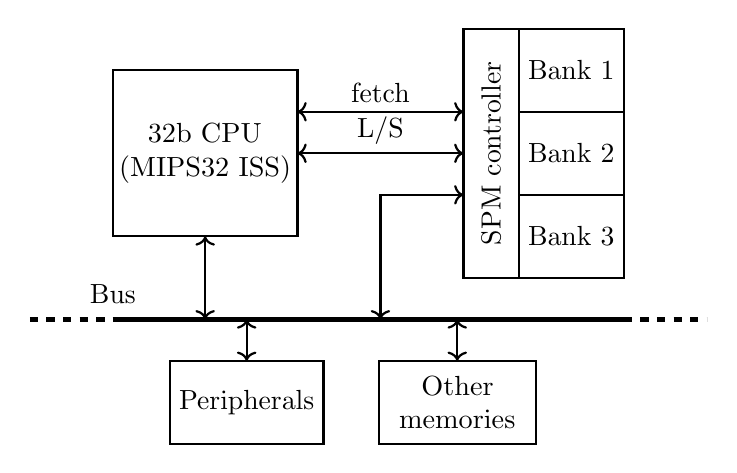
\begin{tikzpicture}[
    outer sep=0pt,node distance=0cm, % allow boxes to touch each other
    mybox/.style={draw,thick,rectangle,align=center},
    ]
    \node (cpu)                                      [mybox,text width=6em,minimum height=6em] {32b CPU\\(MIPS32 ISS)};

    \node (bank2) [node distance=8em,right=of cpu]   [mybox,minimum height=3em] {Bank 2};
    \node (bank1) [above=of bank2]                   [mybox,minimum height=3em] {Bank 1};
    \node (bank3) [below=of bank2]                   [mybox,minimum height=3em] {Bank 3};

    \coordinate [left=2em of bank1.north west] (spmnw);
    \coordinate [left=of bank3.south west]     (spmse);
    \draw [mybox] (spmnw) rectangle (spmse) node [midway,rotate=90] {SPM controller};
    \coordinate (spmw) at (cpu.east -| spmnw); % scratch pad west

    \draw [<->,thick]                 (cpu.east) --                (spmw) node[midway,above] {L/S} ;
    \draw [<->,thick]   ([yshift=1.5em]cpu.east) --  ([yshift=1.5em]spmw) node[midway,above] {fetch} ;
    \draw [<->,thick]     ([yshift=-1.5em]spmw) -| ++(-3em,-4.5em) coordinate (repere1);
    % \draw [fill=red] (repere1) circle (2pt); % debug

    \coordinate (busw) at (repere1 -| cpu.west);  % solid line goes only between 'bus west' and 'bus east'
    \coordinate (buse) at (repere1 -| bank1.east);
    \draw[ultra thick]                     (busw) --              (buse) node [above=.25em, at  start] {Bus};
    \draw[ultra thick,dashed] ([xshift=-3em]busw) --              (busw) ;
    \draw[ultra thick,dashed]              (buse) -- ([xshift=+3em]buse) ;

    \draw [<->,thick] (cpu.south) -- (repere1 -| cpu.south) coordinate (repere2) ;
    % \draw [fill=red] (repere2) circle (2pt); % debug
    \coordinate [below right=1.5em and 1.5em of repere2] (repere3);
    % \draw [fill=red] (repere3) circle (2pt); % debug

    \node (periphs) [below=of repere3] [mybox,minimum height=3em] {Peripherals};
    \draw [<->,thick] (periphs.north) -- (periphs.north |- repere2);

    \node (memory) [right=2em of periphs] [mybox,minimum height=3em,text width=5em] {Other\\memories};
    \draw [<->,thick] (memory.north) -- (memory.north |- repere2);
  \end{tikzpicture}
  \caption{Overview of our simulated platform.}
\end{figure}



% -------------------------------------------------------------------------------------
\subsection{Embedded Software}
% -------------------------------------------------------------------------------------
The platform described above can run bare-metal programs, and some are provided in the repository.
One program correspond to one folder in \lstinline{repository_root/src/platform_tlm/software}.
The target applications will be cross-compiled to MIPS32 and run in the simulator.
Some programs are used for simulator development purposes, others for dynamic memory allocation study.

We list here the programs used for heterogeneous dynamic memory allocation study.


\begin{itemize}
  \item patricia: from MiBench suite
  \item jpeg: from MiBench suite
  \item jpeg2000: from MediaBench 2 suite
  \item dijkstra: from MiBench suite
  \item ecdsa: from mbedTLS test suite
  \item h263: from Mediabench 2 suite
  \item json: based on the use of the Parson library.
\end{itemize}

For a detailed description of the behavior of programs using dynamic memory allocation please refer to reference documents.

\bigskip
We provide the standard library (newlib implementation) to the program without its malloc implementation and provide our own malloc implementation, which is an adaptation of the DLmalloc used in newlib.
The modifications allow us to duplicate data structure describing the heap and so to handle multiple heaps.
The switch between considered heap for an allocation is handled by a novel software module we call the dispatcher, resulting in the software architecture in figure \ref{sw-arch}

\begin{figure}[b]
  \centering
  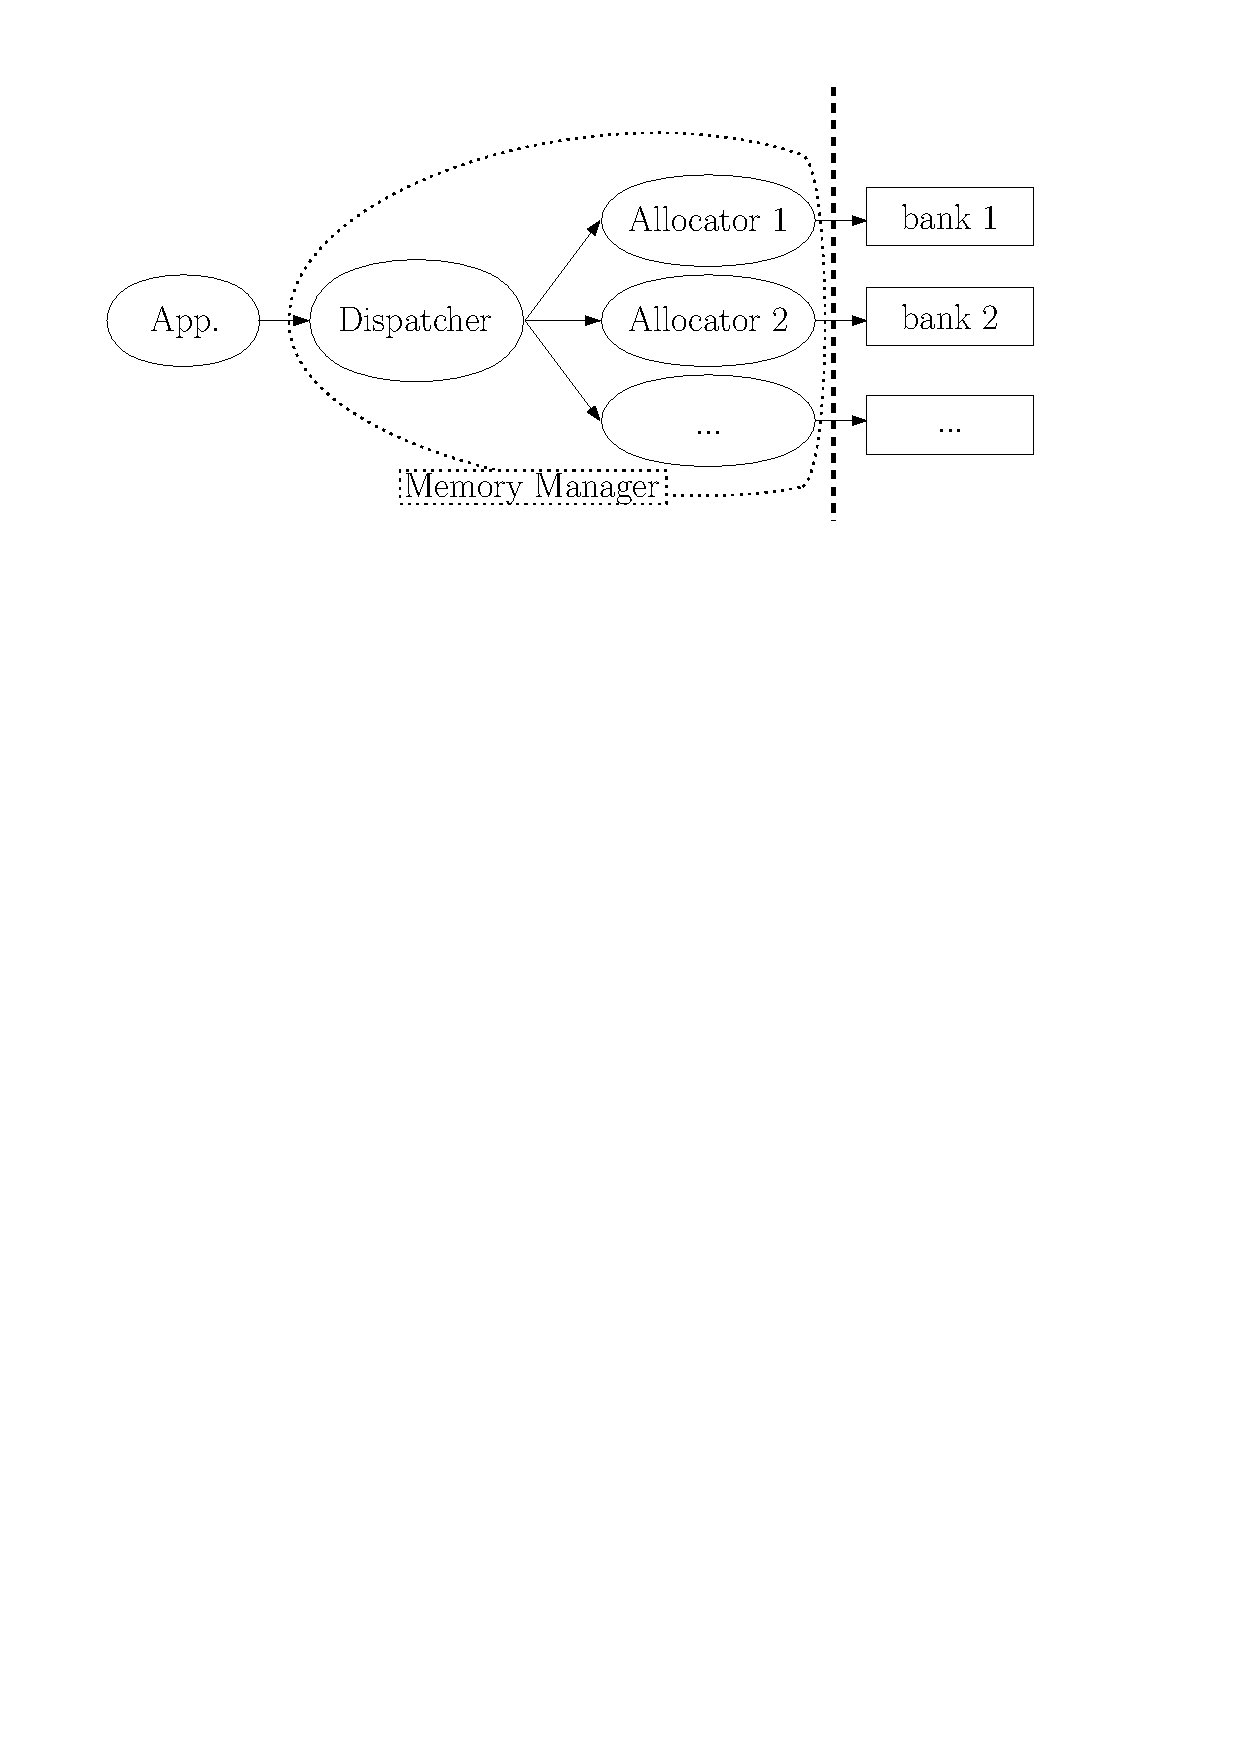
\includegraphics[width=.7\textwidth]{img/sw_hw}
\caption{Software Architecture for Heterogeneous Dynamic Memory Allocation}
\label{sw-arch}
\end{figure}

% -------------------------------------------------------------------------------------
\subsection{Sources Organisation}
% -------------------------------------------------------------------------------------
The project sources are organized as following in \lstinline{src/platform_tlm}:
\begin{itemize}
  \item software: folder containing embedded code, including programs, malloc implementation and dispatcher
  \item logs: contains logs from the last simulator execution
  \item iss: contains the platform description and SystemC main (\lstinline{sc_main.cpp}) along with the Iss
  \item hw\_validation: independent of the simulator, contains the platform for scratchpad memory component unit tests
  \item hardware: contains code for the different simulator components
  \item elf-loader: library for loading embedded software in simulator
\end{itemize}



To change the platform simulated you need to adapt the following files:
\begin{itemize}
  \item sc\_main.cpp: description of the platform, components instantiation and initialization, binding, loading of program and resources, logging system initialization, simulation start and information retrieving.
  \item address\_map.h: describe the physical address map of the simulated platform. This file is used in \lstinline{sc_main.cpp} but is also accessible from the embedded software. This file also defines the latencies of target memory technology used.
  \item platform\_time.h: defines the frequency of simulated core for simulated time measurements
  \item log\_trace.h: log system definitions
\end{itemize}




% =====================================================================================
\section{Build System Setup and Usage}
% =====================================================================================
If you want a native installation please manually follow the steps of the project docker file : \lstinline{src/docker/Dockerfile}.
Otherwise you can build a docker image of the build system and use it in a terminal.
This approach is way more simple and allow to run full experiments.
For development purposes we also describe in this section how to manually build and run the simulator, add new simulated software and adapt the simulated platform.

\bigskip
In order to setup the build system, you need a computer running on a linux distribution with docker and the cloned repository of the project and a valid Cplex installer from IBM.
The executable for Cplex installer is not redistributable and require an account, it is though possible to get a license for free for academic research purposes.


\subsection{Build System Setup}
In a first place you need to build the docker image.
open a terminal in the docker folder located in the Dycton repository (\lstinline{src/docker/Dockerfile}).
You need to copy the Cplex installer in that folder.
Then you can build the docker image using the following command :

\begin{lstlisting}[language=bash]
sudo docker build -t dycton_build_system \
  --build-arg UID=$UID \
  --build-arg CPLEX_INSTALLER=Cplex\_intaller\_name .

\end{lstlisting}
providing your Cplex installer name in parameter instead of "Cplex\_intaller\_name".

\bigskip
This step is long and the build may take a few hours. it requires to have at least 15 Go disk space in / (where the docker images are built by default).
Note that if you need to run this command multiple times it may occupy way more disk space. You can visualize images sizes with \lstinline{sudo docker images} and purge them with \lstinline{sudo docker purge}.
The final image size is around 4 Go


\subsection{Build System Usage}
Once you have build the docker image, you can run a temporary container with the Dycton repository mounted as a docker volume.
This allows you to modify the source code, the configuration files and the simulator outside docker using the container as a build command line terminal.

To launch the container run the following command in a terminal :

\begin{lstlisting}[language=bash]
sudo docker run -it --rm -v /path/to/dycton:/home/build/mounted_repository dycton_build_system
\end{lstlisting}

% -------------------------------------------------------------------------------------
\subsection{Simulator}
% -------------------------------------------------------------------------------------
\subsubsection{Build}
Each simulator built is specific to a particular target application. So if you want to test another application you need to rebuild the simulator.

To build the simulator open the docker build environment in the folder \lstinline{repository_root/src/platform_tlm/iss/}, then use the following command:

\begin{lstlisting}[language=bash]
  build@Dycton_Build_Env(docker)~/mounted_repository/src/platform_tlm/iss$ make DY_SOFT=target_app
\end{lstlisting}

with \lstinline{target_app} the application folder name in \lstinline{repository_root/src/platform_tlm/software/}, if you switch of application built by this command \lstinline{-B} option is mandatory.

\bigskip
The targeted architecture is a simulator run option (\lstinline{-a architecture_number}, see below)

\bigskip
The dataset considered is also a run option (\lstinline{-d dataset_number}


\noindent Strategies used by the dispatcher to allocate in heterogeneous memory (run option \lstinline{-s strategy_name}):
\begin{itemize}
  \item \lstinline{default}: Fast First implementation.
  \item \lstinline{oracle}: Apply a solution given in a file for ILP and Density strategies, require a solution file provided with  \lstinline{-f}
  \item \lstinline{profile}: Profile strategy, require a profile length to take into account with \lstinline{-p}
  \item \lstinline{profile-enhanced} and \lstinline{profile-ilp} are variations of the profile taking into account ILP results for profile construction.
\end{itemize}


\noindent Target memory architecture (run option \lstinline{-a architecture}):
\begin{itemize}
  \item 0: 100\% of heap in fast memory
  \item 1: 75\% of heap in fast memory
  \item 2: 50\% of heap in fast memory
  \item 3: 25\% of heap in fast memory
  \item 4: 10\% of heap in fast memory
  \item 5: 5\% of heap in fast memory
  \item 6: 0\% of heap in fast memory
  \item -2: 100\% of heap in fast and 100\% in slow memory
\end{itemize}

\bigskip
For more information about these option and the different datasets for each application refer to the simulator \lstinline{-h} or \lstinline{--help} options or to the following file: \\\lstinline{repository_root/documents/datasets_characteristics.odt}

% =====================================================================================
\section{Running Experiment Batches}
% =====================================================================================
Exploring the performances of each placement strategy for each application on different repartition of fast and slow memory and for a significant number of input dataset quickly generate a high number of simulator runs.

We propose to use an ensemble of scripts allowing to generate stand alone experiments batches to do this exploration.

note that all the scripts used in this section are located in \lstinline{repository_root/src/scripts/} and can be called with \lstinline{-h} or \lstinline{--help} for a quick description of inputs, outputs and script functionalities.

% -------------------------------------------------------------------------------------
\subsection{Experiment Configuration \texttt{xp\_config.py} and preparation}
% -------------------------------------------------------------------------------------
The \lstinline{xp_config.py} file at repository root describe the experiment batch that the Dycton scripts targets.
In this python file are declared multiple arrays containing the names of target applications, the target architectures, strategies and datasets.
Other options are accessible as the exploration for the profile strategy:
\begin{itemize}
  \item profile\_explo: if set to false stub values defined in the xp\_config.py are used (values provided by default are deprecated, besides they are dependent of target memory technologies)
  \item profile\_high\_resolution: step for profile length exploration (for application with long runtime, may be very costly)
  \item save\_heap\_logs: save all the logs of each execution (not too costly, should stay "True")
\end{itemize}


\bigskip
The script \lstinline{xp_preparation.py} at the repository root will prepare a folder containing all the simulators, datasets, pre-computed profiles required to run the batch of experiments described in xp\_config.py along with a embedded run script.
This allows and targets execution on any x64 linux computer or server (these runs don't require graphical interface).



% -------------------------------------------------------------------------------------
\subsection{Results Synthesis}
% -------------------------------------------------------------------------------------
Once all the simulation runs are complete the results and the logs of the experiments are contained in the \lstinline{result_raw} folder of the experiment batch repertory.

The script \lstinline{dycton_result_synthesis.py}, located in \lstinline{repository_root/src/scripts/} allows to generate one .csv file summarizing the performances of each run.


% -------------------------------------------------------------------------------------
\subsection{Plotting Scripts}
% -------------------------------------------------------------------------------------
The csv file can then be fed to the \lstinline{\repository_root/src/scripts/dycton_plot.py} script.
This script, taking the csv result file as input (\lstinline{-i}) and an application as target (\lstinline{-t}) will plot the application speedup in function of the different considered memory architectures for the different strategies.

Note that this script take into account the \lstinline{xp_config.py} file in the execution directory so it must be executed from the experiment folder.


% =====================================================================================
\section{Example Run}
% =====================================================================================
For this example run we're gonna use one application, and we are going to evaluate ilp, profile and fast first strategies, so our xp\_config.py file is containing these lines :
\begin{lstlisting}[language=bash]
target_sw = ["json_parser", "ecdsa"]
target_hw = ["0", "1", "2", "3", "4", "5", "6"]
target_datasets = [0, 1, 2, 3]
target_strats = ["baseline", "ilp", "ilp_upper_bound","ilp_50", "ilp_85", "density", "density_50",
    "density_85", "profile-switch"]
\end{lstlisting}


Once the \lstinline{xp_config.py} file is correctly configured, you just have to call the experiment batch preparation script \lstinline{xp_prepapration.py} in the repository root.
This must be done from the build environment docker command line as this step will require crosscompilation and Cplex ilp solving.
This step will create a timestamped folder in the repository root embedding the dataset, the simulators, the embedded crosscompiled programs and the script allowing to run all the simulation in batch.

in case of failure of this preparation the folder also contains logs of the different substeps.


\begin{lstlisting}[language=bash]
build@Dycton_Build_Env(docker)~/mounted_repository$ ./xp_preparation.py
Dycton XP preparation script
============================
author: T. Delizy (tristan.delizy@insa-lyon.fr)
2020-05-26_04:31:14.641455


Configuration:
==============
targeted softwares:
  json_parser
  ecdsa

targeted architectures:
  0, 1, 2, 3, 4, 5, 6

targeted strategies for dynamic memory allocation:
  baseline
  ilp
  ilp_upper_bound
  ilp_50
  ilp_85
  density
  density_50
  density_85
  profile-switch

target datasets:
  0, 1, 2, 3

heap memory latencies (cycles) - src/platform_tlm/address_map.h:
  #define MEM_FAST_RLAT (1)
  #define MEM_FAST_WLAT (3)
  #define MEM_SLOW_RLAT (2)
  #define MEM_SLOW_WLAT (30)

profile will be constructed on following datasets:
  4, 5, 6, 7


Starting Xp preparation
=======================
> creating xp folder: dycton_xp_2020-05-26_04:31:14.641455/ ... done.
> prepare clean simulation environment ... done.
> generating reference executions ... done.
> compute profiles for online strategy... done.
> generating architecture descriptors files ... done.
> compute heap placements for offline strategies ... done.
> generate headers from profiles... done.
> generating executable files ... done.
> embedding run script and configuration file ... done.


Summary
=======
preparation completed without errors
to run dycton simulation:
 - go to dycton_xp_2020-05-26_04:31:14.641455/
 - if running on another machine give execution rights to dycton_run_xp.py
 - run dycton_run_xp.py script

results will be stored inside xp folder.
exiting...
\end{lstlisting}

Once the preparation is complete you can launch the experiment batch.
This can be done stand alone in any x64 linux machine (tested on Ubuntu and Debian).
Note that all simulations regarding one program are launched simultaneously, and depending on the number of architectures, datasets and strategies under test that can spawn more than hundred processes.

All spawned processes are 12-nice, allowing concurrent tasks to execute.

The run script to launch is \lstinline {dycton_run_xp.py}, it is copied into the experiment folder during preparation and use the \lstinline{xp_config.py} file, also embedded in the experiment folder during the preparation.

\begin{lstlisting}[language=bash]
./dycton_run_xp.py
config file loaded.
Dycton experiment run script
================================================================================
author: T. Delizy (tristan.delizy@insa-lyon.fr)
2020-05-26 12:11:42.211947
end of experiment run, exiting...
printing the run dict:
{ 'dijkstra': [],
  'ecdsa': [ { 'cmd': [ 'nice',
                        '-12',
                        './ecdsa_sim.x',
                        '-c',
                        '-a',
                        '0',
                        '-d',
                        '0'],
               'name': 'ecdsa_arch0_d0_baseline_run',
               'path': './xp_run/ecdsa_arch0_d0_baseline_run/',
               'process': <subprocess.Popen object at 0x7f6f248791c0>,
               'ret': 0},
             { 'cmd': [ 'nice',
                        '-12',
                        './ecdsa_sim.x',
                        '-c',
                        '-a',
                        '0',
                        '-d',
                        '1'],
               'name': 'ecdsa_arch0_d1_baseline_run',
               'path': './xp_run/ecdsa_arch0_d1_baseline_run/',
               'process': <subprocess.Popen object at 0x7f6f10b463d0>,
               'ret': 0},
               ...
\end{lstlisting}

The run script is not very verbose. To follow the experiment progress use \lstinline{ps aux} command, greping for your user name or the target application. One other problem that may arise is a low disk space in the partition where the experiment is run as the scripts will copy a clean environment for each run. These environment are deleted at the end of the runs.

\bigskip
Once all the simulation are done, retrieve the batch folder and execute the \lstinline{dycton_result_synthesis.py} inside of it to summarize the runs performances into one csv file.

\begin{lstlisting}[language=bash]
  python ../src/scripts/dycton_result_synthesis.py -i results_raw/
  Result synthesis (CSV) construction from experiment logs
  ========================================================
  author: T. Delizy (tristan.delizy@insa-lyon.fr)
  2020-06-12 10:21:07.523932
  input path: results_raw/
  	 ecdsa_arch0_d0_baseline_run ok.
  	 ecdsa_arch0_d1_baseline_run ok.
  	 ecdsa_arch0_d2_baseline_run ok.
  	 ecdsa_arch0_d3_baseline_run ok.
  	 ecdsa_arch1_d0_baseline_run ok.
  	 ecdsa_arch1_d0_density_50_run ok.
  	 ecdsa_arch1_d0_density_85_run ok.
...
     json_parser_arch6_d1_baseline_run ok.
     json_parser_arch6_d2_baseline_run ok.
     json_parser_arch6_d3_baseline_run ok.
success : experiment run without errors.
\end{lstlisting}


The csv file contains one line for each simulator run.
The second column contains the return code of the simulation, allowing to detect here if a run had a problem.
If it occurs you can then access the logs of this particular simulation in \lstinline{experiment_batch_generated_folder/results_raw/logs/run_name/logs/}.
However, for debug purposes you should re-run this execution locally and manually.

\begin{lstlisting}
  #experience;return_code;final cycles;allocator cycles;fallback
  ecdsa_arch0_d0_baseline_run;0;103272230;11374548;0
  ecdsa_arch0_d1_baseline_run;0;102783827;11329656;0
  ecdsa_arch0_d2_baseline_run;0;103368317;11372760;0
  ...
\end{lstlisting}

This csv file can then be feed to the \lstinline{dycton_plot.py} script which will plot the graphs presenting the performances of each strategy.


\begin{lstlisting}[language=bash]
  $ python ../src/scripts/dycton_plot.py -i results/result_synthesis.csv
  Dycton plot script
  ================================================================================
  author: T. Delizy (tristan.delizy@insa-lyon.fr)
  2020-06-12 12:04:49.043407

  > command line arguments processing ...  done.

  > experiment configuration file loading ... done.

  > loaded config :
  	 Apps : ['json_parser', 'ecdsa']
  	 Archis :  ['0', '1', '2', '3', '4', '5', '6']
  	 Strategies :  ['baseline', 'ilp', 'ilp_upper_bound', 'ilp_50', 'ilp_85',
                    'density', 'density_50', 'density_85', 'profile']
  	 Datasets :  [0, 1, 2, 3]
  > constructing result structure ...  done.

  ================================================================================
  data retrieving and preparation
  ================================================================================
  > parsing allocation log ...  done.

  > start of parsed data:
  ('experience', 'return_code', 'final_cycles', 'allocator_cycles', 'fallback')
  [('ecdsa_arch0_d1_baseline_run', 0, 102783827, 11329656,  0.    )
   ('ecdsa_arch0_d2_baseline_run', 0, 103368317, 11372760,  0.    )
   ('ecdsa_arch0_d3_baseline_run', 0, 102933365, 11346438,  0.    )
   ('ecdsa_arch1_d0_baseline_run', 0, 111250196, 13316072, 22.6147)
   ('ecdsa_arch1_d0_density_50_run', 0, 119250558, 14215639,  0.    )]
  ...

  > populating result structure...  done.

  ================================================================================
  plotting json_parser
  ================================================================================


  arch =  [100, 75, 50, 25, 10, 5, 0]
  arch names =  ['100%', '75%', '50%', '25%', ' 10%', '5%', '0%']
  strats = ['baseline', 'ilp', 'ilp_upper_bound', 'ilp_50', 'ilp_85', 'density',
            'density_50', 'density_85', 'profile']
  qt5ct: using qt5ct plugin
  ================================================================================
  plotting ecdsa
  ================================================================================


  arch =  [100, 75, 50, 25, 10, 5, 0]
  arch names =  ['100%', '75%', '50%', '25%', ' 10%', '5%', '0%']
  strats = ['baseline', 'ilp', 'ilp_upper_bound', 'ilp_50', 'ilp_85', 'density',
            'density_50', 'density_85', 'profile']

\end{lstlisting}


The runs of these simulations yield two plots, one by target application.
These plots show the reduction of execution time in cycle in function of the proportion of the heap in fast memory.

Each curve describe the performance of one dispatch strategy.
Each point in these graphs represents the average over multiple datasets of the execution time reduction compared to an execution where all the heap is located in slow memory.
Error bars correspond to the minimum and maximum performances observed over the different datasets.
The figure \ref{result_plots} present the example run result plots.

\begin{figure}[h]
  \centering
  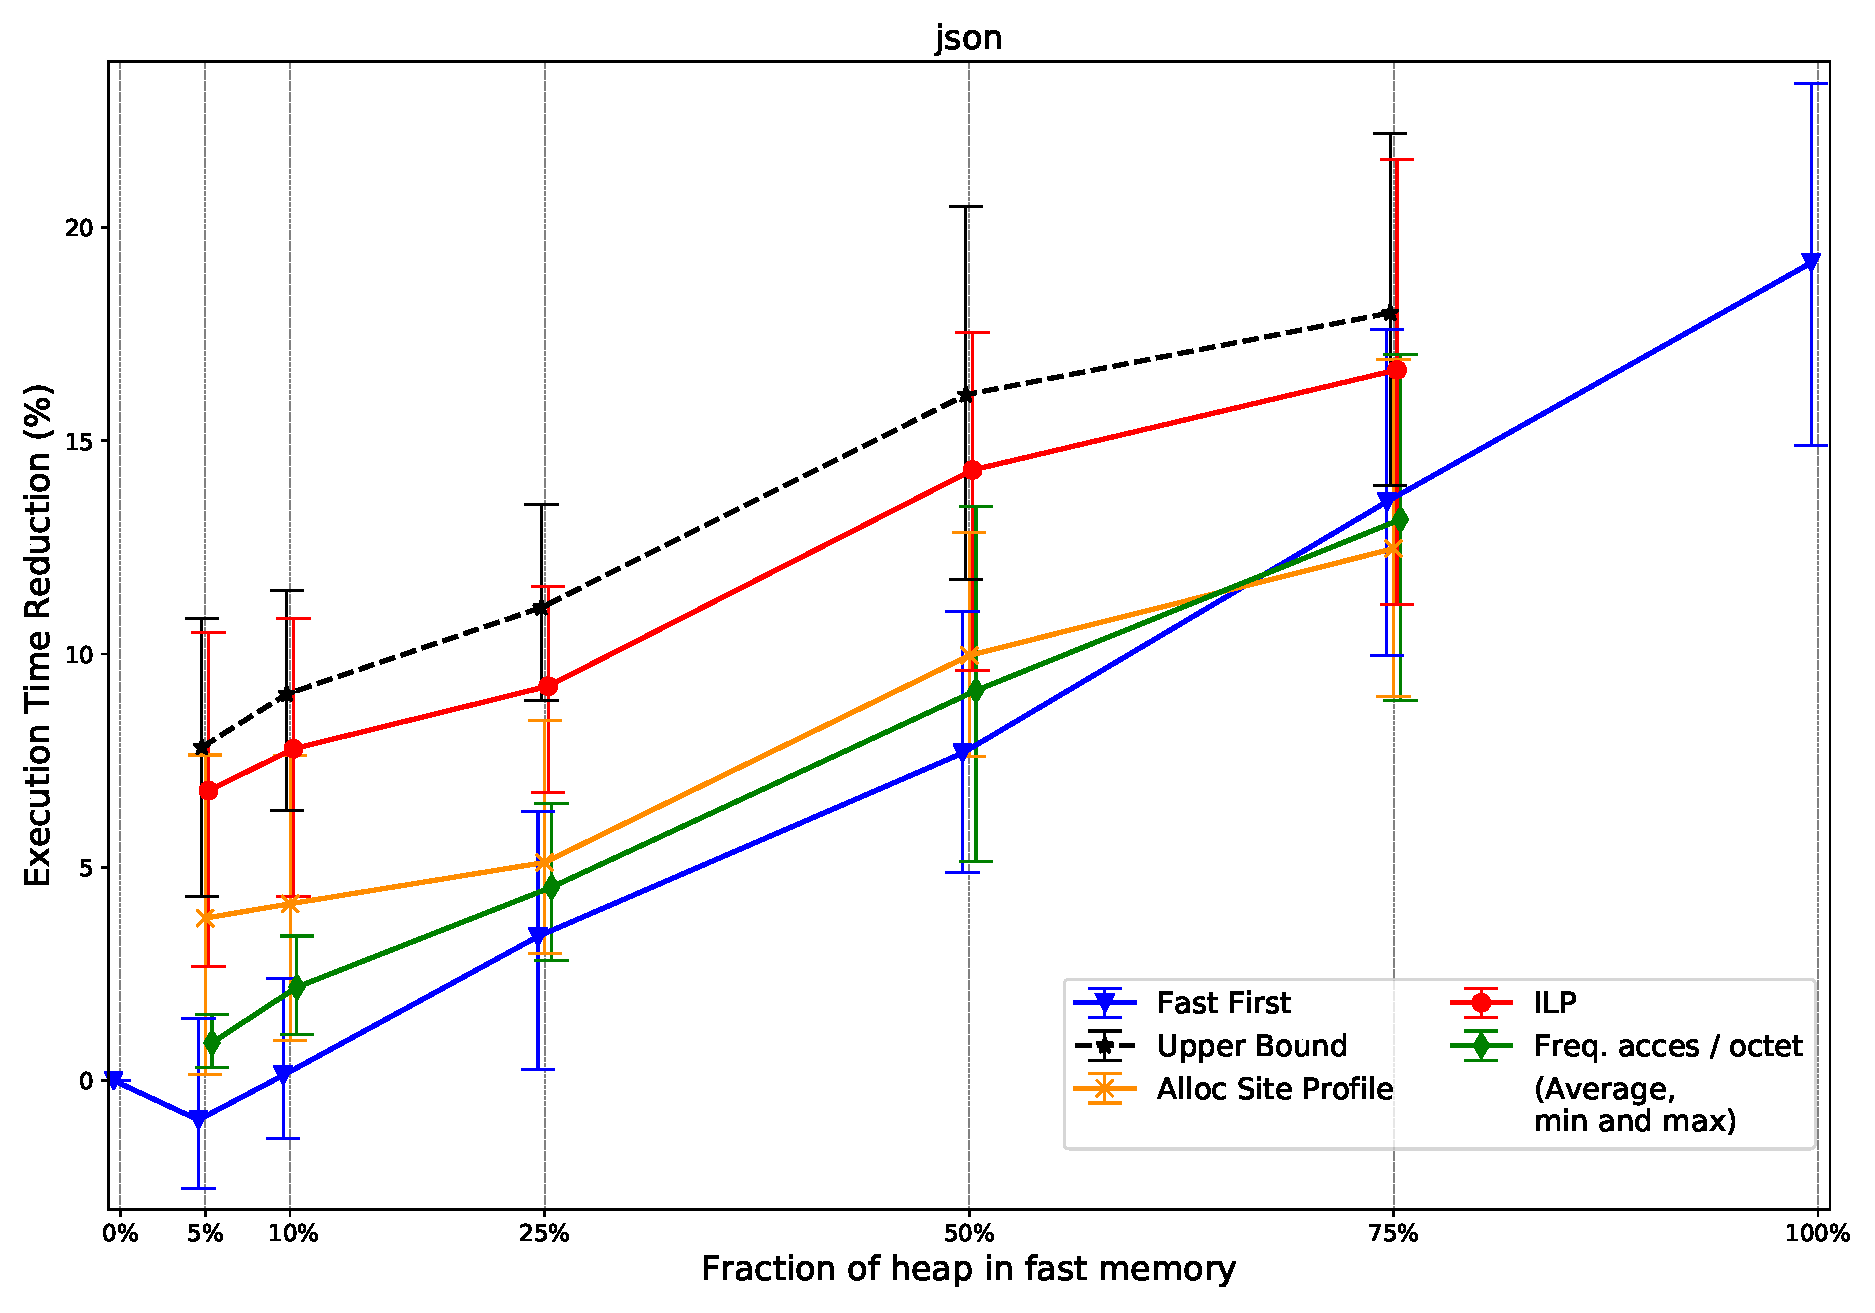
\includegraphics[width=.6\textwidth]{img/json_parser_A(0-1-2-3-4-5-6)D(0-1-2-3)S(ff-ilp-freq-prof).pdf}
  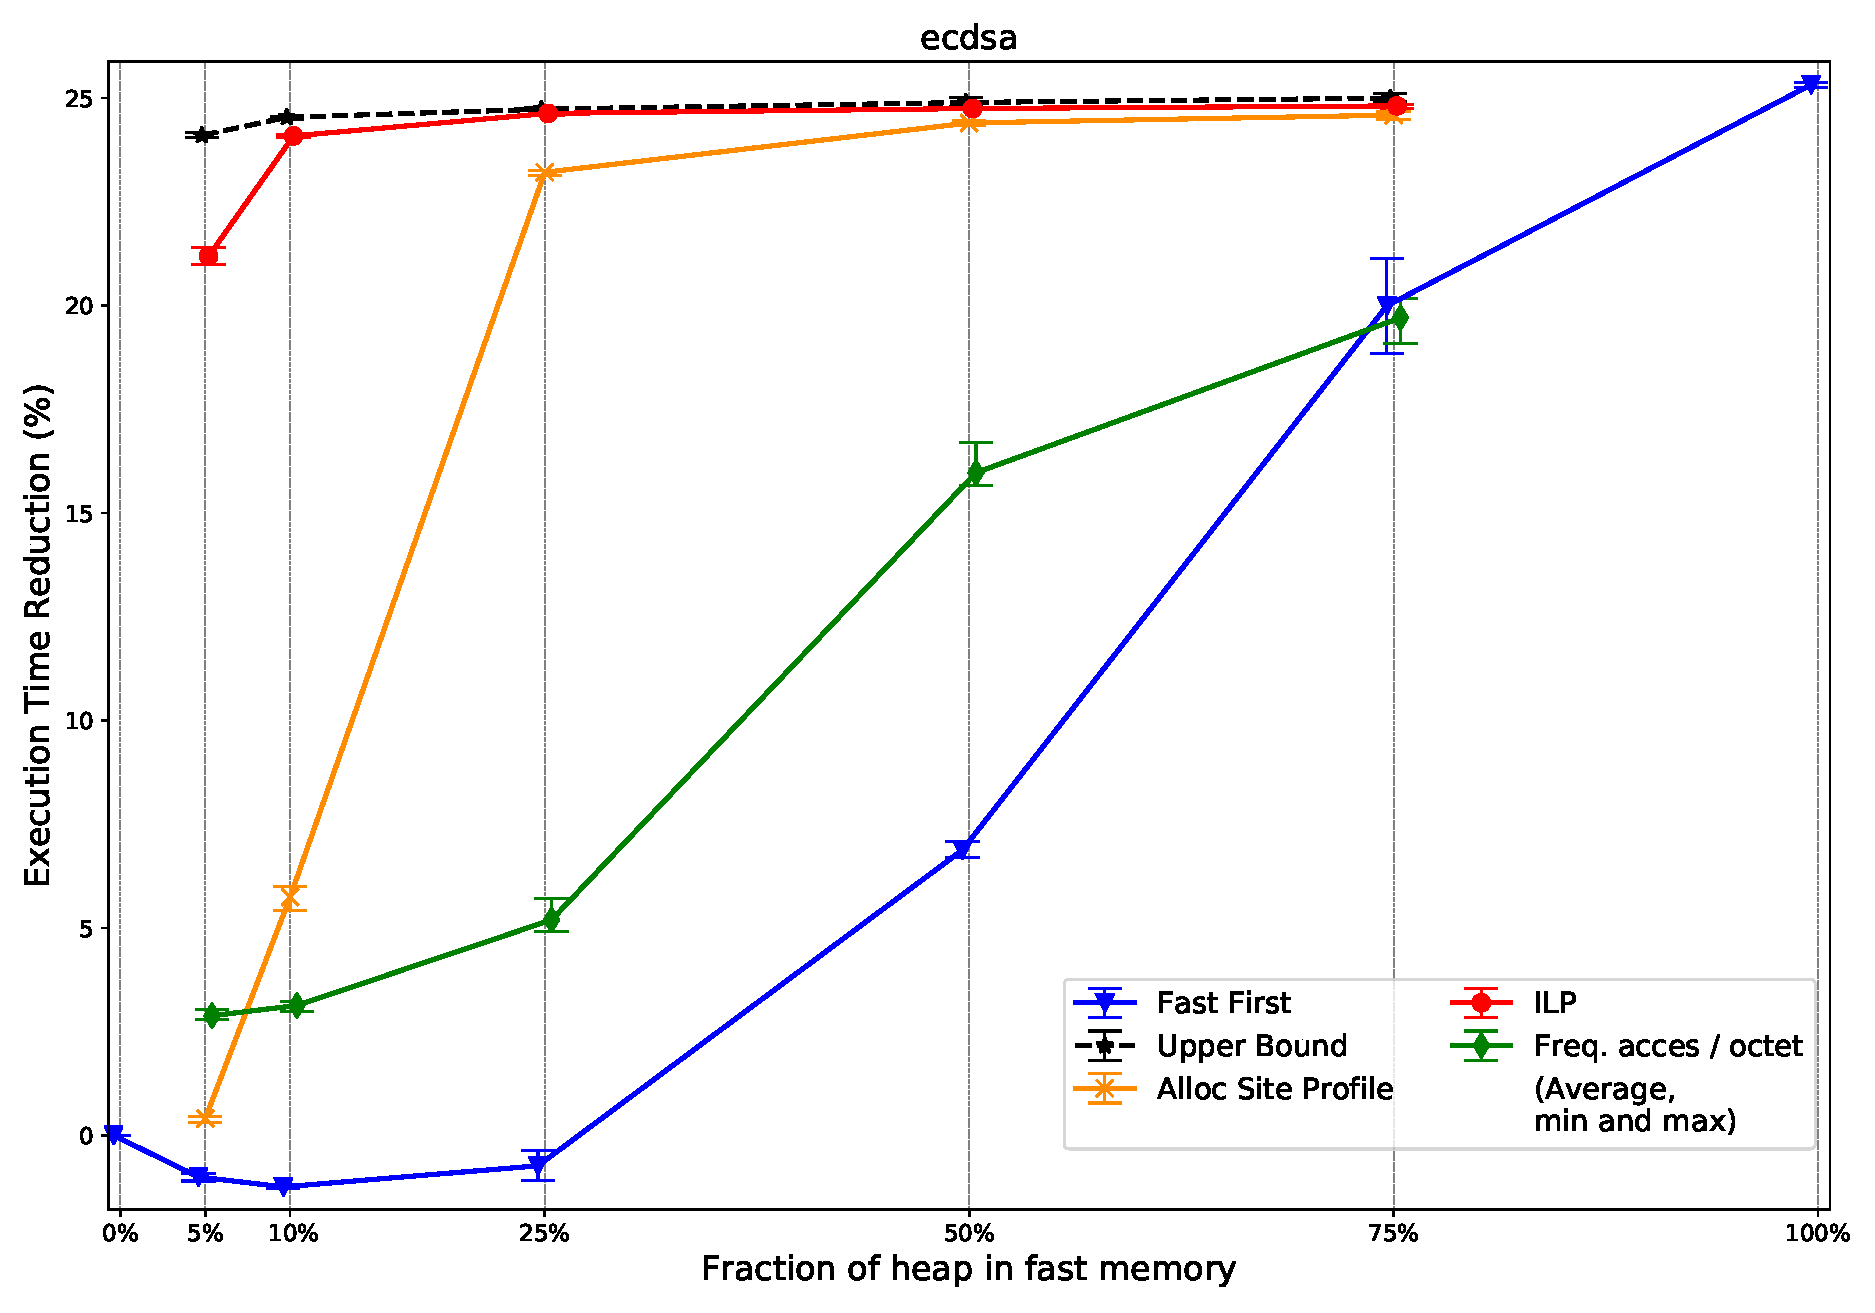
\includegraphics[width=.6\textwidth]{img/ecdsa_A(0-1-2-3-4-5-6)D(0-1-2-3)S(ff-ilp-freq-prof).pdf}
\caption{Example run results}
\label{result_plots}
\end{figure}



\end{document}
